% Source with record ids (@123) in \cite{}; build_tex.py turns them into verified BibTeX keys -> main.tex
\documentclass[preprint,12pt]{elsarticle}
\usepackage[utf8]{inputenc}
\usepackage[T1]{fontenc}
\usepackage{amsmath,amssymb,booktabs,longtable,array,graphicx,xcolor,multirow,url}
\usepackage[hidelinks]{hyperref}
\usepackage{tikz}
\renewcommand{\topfraction}{0.9}\renewcommand{\bottomfraction}{0.8}\renewcommand{\textfraction}{0.1}\renewcommand{\floatpagefraction}{0.7}\setcounter{topnumber}{3}\setcounter{bottomnumber}{2}\setcounter{totalnumber}{5}
\usetikzlibrary{positioning,arrows.meta,fit}
\newcommand{\nQueries}{42}
\newcommand{\nPages}{53}
\newcommand{\nRetrieved}{5{,}047}
\newcommand{\nUnique}{3{,}915}
\newcommand{\nWithAbs}{3{,}677}
\newcommand{\nStageOne}{4{,}740}
\newcommand{\nSelected}{250}
\newcommand{\nVerified}{236}
\newcommand{\nDropped}{14}
\newcommand{\nAudit}{60}
\newcommand{\nAuditCand}{67}
\newcommand{\nAuditDropped}{7}
\newcommand{\nGeofenceBucket}{358}
\newcommand{\nAttBucket}{2{,}654}
\newcommand{\nLpwanBucket}{1{,}393}
\newcommand{\nRescreen}{21}
\newcommand{\nRescreenVer}{19}
\newcommand{\nAuditLang}{8}
\newcommand{\nPriorSel}{29}
\newcommand{\nSources}{7}
\newcommand{\srcPhrase}{7 sources: four open ones (OpenAlex, Crossref, arXiv and Semantic Scholar) and Scopus, Web of Science and IEEE Xplore}
\newcommand{\srcMissing}{Scopus, Web of Science and IEEE Xplore were searched through exports on 11 November 2026 (institutional access or free search); none of the three major proprietary indexes is missing.}
\newcommand{\srcThreat}{Coverage of the proprietary databases depends on our queries and on the exports we obtained.}
\newcommand{\srcQueryExtra}{, 8 Scopus, 6 Web of Science, 5 IEEE Xplore}
\newcommand{\srcRecordsExtra}{, 4{,}784 Scopus, 1{,}073 Web of Science, 103 IEEE Xplore}
\newcommand{\srcFlow}{OpenAlex 5{,}047, Crossref 2{,}400, arXiv 49, S2 100, Scopus 4{,}784, Web of Science 1{,}073, IEEE Xplore 103}
\newcommand{\srcOA}{5{,}047}
\newcommand{\srcCR}{2{,}400}
\newcommand{\srcAX}{49}
\newcommand{\srcSS}{100}
\newcommand{\nQueriesOA}{42}
\newcommand{\nQueriesCR}{18}
\newcommand{\nQueriesAX}{6}
\newcommand{\nQueriesSS}{1}
\newcommand{\nQueriesAll}{86}
\newcommand{\totRetrieved}{13{,}556}
\newcommand{\unionUnique}{9{,}808}
\newcommand{\newOther}{5{,}893}
\newcommand{\dupRemoved}{3{,}748}
\newcommand{\exclStageOne}{5{,}068}
\newcommand{\exclStageTwo}{4{,}490}
\newcommand{\nAuditOnlyOther}{0}
\newcommand{\aSecond}{45}
\newcommand{\pSecond}{75}
\newcommand{\aFace}{28}
\newcommand{\pFace}{47}
\newcommand{\aBio}{21}
\newcommand{\pBio}{35}
\newcommand{\aQr}{14}
\newcommand{\pQr}{23}
\newcommand{\aRfid}{8}
\newcommand{\pRfid}{13}
\newcommand{\aCircle}{14}
\newcommand{\pCircle}{23}
\newcommand{\aPoly}{4}
\newcommand{\pPoly}{7}
\newcommand{\aSpoof}{28}
\newcommand{\pSpoof}{47}
\newcommand{\aQuant}{23}
\newcommand{\pQuant}{38}
\newcommand{\aMetric}{6}
\newcommand{\pMetric}{10}
\newcommand{\aLocerr}{4}
\newcommand{\pLocerr}{7}
\newcommand{\aPriv}{3}
\newcommand{\pPriv}{5}
\newcommand{\aLpwan}{0}
\newcommand{\pLpwan}{0}
\newcommand{\aDeployed}{20}
\newcommand{\pDeployed}{33}
\newcommand{\aEarly}{5}
\newcommand{\aYtwentythree}{6}
\newcommand{\aYtwentyfour}{6}
\newcommand{\aYtwentyfive}{17}
\newcommand{\aYtwentysix}{26}
\newcommand{\aRecent}{43}
\newcommand{\pRecent}{72}
\newcommand{\nPriorGps}{6}

\newcommand{\nOthers}{2{,}326}
\newcommand{\modFace}{922}
\newcommand{\modAccNFace}{207}
\newcommand{\modAccMedFace}{95.7}
\newcommand{\modAccPctFace}{22}
\newcommand{\modSpoofPctFace}{30}
\newcommand{\modBio}{255}
\newcommand{\modAccNBio}{31}
\newcommand{\modAccMedBio}{95.6}
\newcommand{\modAccPctBio}{12}
\newcommand{\modSpoofPctBio}{33}
\newcommand{\modRfid}{171}
\newcommand{\modAccNRfid}{8}
\newcommand{\modAccMedRfid}{93.5}
\newcommand{\modAccPctRfid}{5}
\newcommand{\modSpoofPctRfid}{20}
\newcommand{\modNfc}{39}
\newcommand{\modAccNNfc}{1}
\newcommand{\modAccMedNfc}{--}
\newcommand{\modAccPctNfc}{3}
\newcommand{\modSpoofPctNfc}{33}
\newcommand{\modBle}{47}
\newcommand{\modAccNBle}{0}
\newcommand{\modAccMedBle}{--}
\newcommand{\modAccPctBle}{0}
\newcommand{\modSpoofPctBle}{21}
\newcommand{\modQr}{120}
\newcommand{\modAccNQr}{4}
\newcommand{\modAccMedQr}{--}
\newcommand{\modAccPctQr}{3}
\newcommand{\modSpoofPctQr}{27}
\newcommand{\modWifi}{14}
\newcommand{\modAccNWifi}{1}
\newcommand{\modAccMedWifi}{--}
\newcommand{\modAccPctWifi}{7}
\newcommand{\modSpoofPctWifi}{14}
\newcommand{\modUnspec}{758}
\newcommand{\modAccNUnspec}{26}
\newcommand{\modAccMedUnspec}{97.5}
\newcommand{\modAccPctUnspec}{3}
\newcommand{\modSpoofPctUnspec}{13}
\newcommand{\nOthersRecent}{2{,}039}
\newcommand{\cmpGacc}{13}
\newcommand{\cmpOacc}{13}
\newcommand{\cmpGsample}{13}
\newcommand{\cmpOsample}{7}
\newcommand{\cmpGspoof}{45}
\newcommand{\cmpOspoof}{26}
\newcommand{\cmpGpriv}{5}
\newcommand{\cmpOpriv}{5}
\newcommand{\nCore}{6}
\newcommand{\nOA}{48}
\newcommand{\nGeoAll}{358}
\newcommand{\domLoraTotal}{12}
\newcommand{\domLoraLive}{4}
\newcommand{\domAtt}{76}
\newcommand{\domPctAtt}{21}
\newcommand{\domHealth}{36}
\newcommand{\domPctHealth}{10}
\newcommand{\domLive}{27}
\newcommand{\domPctLive}{8}
\newcommand{\domAvi}{38}
\newcommand{\domPctAvi}{11}
\newcommand{\domVeh}{43}
\newcommand{\domPctVeh}{12}
\newcommand{\domMkt}{58}
\newcommand{\domPctMkt}{16}
\newcommand{\domSafe}{39}
\newcommand{\domPctSafe}{11}
\newcommand{\domOther}{41}
\newcommand{\domPctOther}{11}

\newcommand{\ftN}{17}
\newcommand{\ftTried}{60}
\newcommand{\ftNoOA}{12}
\newcommand{\ftShort}{13}
\newcommand{\ftErr}{7}
\newcommand{\ftPct}{47}
\newcommand{\ftAllN}{28}
\newcommand{\ftCodes}{119}
\newcommand{\ftCcPct}{28}
\newcommand{\ftQone}{2}
\newcommand{\ftQtwo}{3}
\newcommand{\ftQthree}{2}
\newcommand{\ftQfour}{0}
\newcommand{\ftQfive}{0}
\newcommand{\ftQsix}{0}
\newcommand{\ftQseven}{5}
\newcommand{\ftAbsQone}{1}
\newcommand{\ftAbsQtwo}{3}
\newcommand{\ftScoreZero}{10}
\newcommand{\ftScoreOne}{4}
\newcommand{\ftScoreTwo}{1}
\newcommand{\ftScoreThree}{2}
\newcommand{\ftScoreMax}{3}
\newcommand{\ftScoreAtLeastTwo}{3}
\newcommand{\ftBestCites}{\cite{amoanu2026session,kumar2026geosecure}}
\newcommand{\agN}{9}
\newcommand{\agNAll}{14}
\newcommand{\agJ}{63}
\newcommand{\agPct}{98}
\newcommand{\agKappa}{0.90}
\newcommand{\ftLicCC}{17}
\newcommand{\ftLicNone}{11}
\newcommand{\humanSentence}{}
\newcommand{\humanThreat}{The first coder applied all rules and the second coder was an AI model that saw only snippets. One author (LHP) then read each of the \ftN{} full texts and checked every full-text code against the paper, changing none of the \ftCodes{} codes; because that author is one of us and saw the codes first, this is a check and not an independent second coding, and no person outside the author team re-coded the papers. The abstract-level codes were not re-checked by a person.}
\newcommand{\coderAbs}{The first coder applied all rules and a second coder, also an AI model, re-coded a sample of full texts from snippets; one author then checked all \ftN{} full-text codes against the papers and changed none of them, and no person outside the author team re-coded them.}

\newcommand{\hfN}{60}
\newcommand{\hfConsent}{0}
\newcommand{\hfDevBind}{3}

\biboptions{sort&compress}
\journal{Internet of Things}
\newcommand{\todo}[1]{\textcolor{red}{[#1]}}
\newcolumntype{L}[1]{>{\raggedright\arraybackslash}p{#1}}

\emergencystretch=3em
\begin{document}
\begin{frontmatter}
\title{Presence sensing with GPS geofences and LPWAN for automatic attendance: a mapping study, an evidence audit and a research agenda}
\author[vit]{Dhanisha S}
\author[vit]{Lakshmi Harika P}
\author[vit]{Adesh Kanna P}
\author[vit]{Ananyaa S}
\affiliation[vit]{organization={Vellore Institute of Technology, Chennai},department={School of Computer Science and Engineering},country={India}}

\begin{abstract}
Automatic attendance is moving from cards and cameras to phones and radios. Geofencing, which marks a person present when a location fix falls inside a boundary, is now common in attendance applications, and LoRa radios can carry the same logic to devices without a phone. We ran \nQueriesAll{} documented queries on \nSources{} sources, selected \nSelected{} records and verified \nVerified{} against DOI registries. Earlier attendance reviews are mostly organised by sensing modality, and the one geolocation-based review we found is a short narrative without an evidence audit. We audited \nAudit{} geofence-based attendance systems from their abstracts and, for the \ftN{} whose open-access copy carries a Creative Commons licence, from their full texts (AI second-coder agreement on \agN{} papers: $\kappa=\agKappa$). In the full texts, \ftQtwo{} of \ftN{} measure the geofence decision, \ftQone{} handle location error, \ftQthree{} test an attack, none reports energy and none uses LoRa; \hfConsent{} of \hfN{} abstracts mention consent. Thin reporting is not unique to geofencing: of \nOthersRecent{} other attendance systems since 2018, \cmpOacc\% give an accuracy figure in the abstract, against \cmpGacc\% of the geofence systems. We propose a seven-item reporting checklist; \ftScoreZero{} of the \ftN{} papers meet none of its items. A companion simulation on real GPS tracks shows the cost of the gaps: a plain radius test gives 0.455 false events per track-hour, hysteresis removes about 94\% of them, and class changes cut the capacity of one LoRa gateway by about 15\%. We close with a research agenda.
\end{abstract}

\begin{highlights}
\item Reproducible mapping of GPS and LPWAN attendance work, DOI-verified references
\item Full-text audit: boundary error and location attacks are rarely tested
\item Thin reporting is field-wide: face, RFID and QR systems show the same gap
\item No audited system uses LoRa; none of the abstracts mentions consent
\item Seven-item reporting checklist for presence-sensing papers
\end{highlights}

\begin{keyword}
attendance \sep geofencing \sep GPS \sep LoRa \sep LPWAN \sep Internet of Things \sep location privacy \sep survey
\end{keyword}
\end{frontmatter}

%--------------------------------------------------------------------
\section{Introduction}
Calling a register in a large class can take minutes, and paper registers invite proxy marks. Automatic alternatives have multiplied: cards and tags \cite{@36,@86,@210}, Bluetooth beacons \cite{@159,@165}, fingerprint scanners \cite{@47,@168}, face recognition \cite{@16,@33,@78} and QR codes \cite{@61}. Each swaps one chore for another, because someone must carry the card, stand at the reader, face the camera or share a code.

Geofencing removes the reader. A phone or a small tracker reports its position, and software marks the person present when the position falls inside a boundary around the classroom, campus or worksite. The idea is older than attendance applications \cite{reclus2009geofencing,@175}, and attendance is now its largest single use among the records we retrieved (Section~\ref{sec:domain}). A second line of work attaches the same logic to LoRa nodes, so that presence or boundary breaches can be reported from devices without a phone or Wi-Fi \cite{@357,@1235}. Both lines depend on things the attendance literature rarely examines: how wrong a location fix can be, how long a battery lasts when fixes are frequent, and how many reports a radio network can carry when a lecture hall empties at once.

Existing reviews do not examine these questions. Table~\ref{tab:prior} lists the \nPriorSel{} attendance reviews that our search found. Most are organised by sensing modality, and only \nPriorGps{} of them mention GPS or geofencing in the abstract, in passing. One, returned only by IEEE Xplore and Scopus and by none of the open sources, is titled for geolocation-based attendance \cite{@3025}. Its text on the publisher's page is a short narrative review of GPS and geofence attendance systems, with GPS inaccuracy, spoofing, privacy and battery use mentioned briefly, no stated search protocol and no audit of what the studies report. We ask:
\begin{description}
\item[RQ1] Which sensing technologies support automatic attendance, and how do geofence and LPWAN approaches differ from them?
\item[RQ2] What evidence do geofence-based attendance systems report, and how do they treat location uncertainty?
\item[RQ3] Is thin reporting specific to geofencing, or common to attendance systems?
\item[RQ4] What do the energy, LPWAN and privacy literatures imply for deploying such systems at scale, and what is missing?
\end{description}

\paragraph{Contributions} (i) A reproducible mapping study over \srcPhrase{}, with every query, count and screening rule published. (ii) A taxonomy of attendance sensing that places GPS geofences and LPWAN nodes beside the better-known modalities, with a quantitative look at reporting practice by modality (Section~\ref{sec:tax}). (iii) An evidence audit of \nAudit{} geofence-based attendance systems from abstracts, with a full-text check of the open-access subset, a blind second coder and a comparison group of \nOthersRecent{} other attendance systems (Section~\ref{sec:audit}). (iv) A cross-layer synthesis of location uncertainty, sampling energy, LPWAN scalability and privacy (Sections~\ref{sec:unc}--\ref{sec:priv}), illustrated by a short summary of a companion simulation (Section~\ref{sec:case}). (v) A people-in-the-loop analysis of privacy, regulation and security, with design requirements (Section~\ref{sec:priv}), and a seven-item minimum reporting checklist scored on the full texts (Section~\ref{sec:checklist}). (vi) A research agenda (Section~\ref{sec:agenda}). We call the work a mapping study, not a systematic review: selection used ranked retrieval and documented rules, not full-text appraisal of every candidate.

\begin{table}[tbp]\centering\footnotesize
\caption{Earlier attendance reviews found by the search. ``GPS/geofence'' = the abstract mentions it. One review \cite{gupta2025geolocation} is centred on geolocation-based attendance; it was returned only by IEEE Xplore and Scopus, its abstract mentions neither GPS nor geofencing, and its text on the publisher's page has four sections and no stated search protocol. No other review in this set is centred on geofencing, GPS or LPWAN presence sensing.}\label{tab:prior}
\begin{tabular}{@{}L{3.3cm}llL{4.0cm}c@{}}\toprule Ref. & Year & Type & Focus & GPS/geofence \\ \midrule
\cite{binmohdnasir2015review} & 2015 & review & NFC & no \\
\cite{hoo2019biometric} & 2019 & review & Biometric (hardware) & no \\
\cite{x2020rfid} & 2020 & review & RFID & no \\
\cite{alagasan2021review} & 2021 & review & Fingerprint, iris, RFID, GPS & yes \\
\cite{anshari2021face} & 2021 & systematic & Face recognition & no \\
\cite{bai2021survey} & 2021 & review & General (real-time automated) & no \\
\cite{raj2021attendance} & 2021 & review & Computer vision, biometrics & no \\
\cite{x2021automation} & 2021 & review & Biometrics, RFID, BLE, GPS, QR & yes \\
\cite{budiman2023student} & 2022 & systematic & Face recognition & no \\
\cite{modak2022systematic} & 2022 & systematic & Face recognition & yes \\
\cite{abidemi2023attendance} & 2023 & review & IoT, blockchain, AI & no \\
\cite{anon2023smart} & 2023 & review & Smart campus, general & no \\
\cite{ardebili2022comprehensive} & 2023 & systematic & Employee, cloud-based & no \\
\cite{barbosadasilva2023student} & 2023 & systematic & Bluetooth & no \\
\cite{ishaq2023based} & 2023 & systematic & RFID & no \\
\cite{saxena2023review} & 2023 & review & Face recognition & no \\
\cite{alshamsi2024computer} & 2024 & review & Computer vision & no \\
\cite{anon2024review} & 2024 & review & General & no \\
\cite{muslim2024smart} & 2024 & systematic & Smart card & no \\
\cite{shrivastav2024systematic} & 2024 & systematic & General & no \\
\cite{x2024comprehensive} & 2024 & review & General & no \\
\cite{dliyaulhaq2025systematic} & 2025 & systematic & AppSheet apps & yes \\
\cite{gupta2025geolocation} & 2025 & review & Geolocation, geofencing (short narrative) & no \\
\cite{jodihendrawan2025code} & 2025 & systematic & QR code & yes \\
\cite{x2025which} & 2025 & systematic & General (class attendance) & no \\
\cite{chakraborty2026comprehensive} & 2026 & review & Machine learning & no \\
\cite{fatikha2026utilization} & 2026 & review & Facial biometrics & no \\
\cite{ohal2026review} & 2026 & review & QR + geofencing; performance & yes \\
\cite{patel2026comprehensive} & 2026 & review & Face recognition & no \\
\bottomrule\end{tabular}\end{table}


%--------------------------------------------------------------------
\section{Survey methodology}\label{sec:method}
We report the method following the PRISMA extension for scoping reviews \cite{tricco2018prismascr}, the nearest reporting guideline to a mapping study, and draw the flow of records after the PRISMA 2020 diagram \cite{page2021prisma}. The completed checklist is a supplementary file. No protocol was registered before the search; the queries, rules and counts are published instead.

\subsection{Sources and search}
We used four open sources that need no login: OpenAlex, Crossref, arXiv and Semantic Scholar. OpenAlex was the main source because it returns abstracts and metadata for the same query repeatably. Crossref and arXiv were added to test whether another index would surface systems OpenAlex missed. Semantic Scholar throttled anonymous access, so only one query returned (it overlapped with OpenAlex in 87 of 100 records). \srcMissing{} The open-source queries ran on 4 November 2026. In all there were \nQueriesAll{} query runs (\nQueriesOA{} OpenAlex, \nQueriesCR{} Crossref, \nQueriesAX{} arXiv, \nQueriesSS{} Semantic Scholar\srcQueryExtra{}; Appendix~\ref{app:queries}) over articles, reviews, preprints, book chapters and conference papers from 2005. The queries covered geofencing and attendance, GPS and LoRa tracking, competing attendance technologies, LoRa scalability and security, GPS energy and accuracy, location privacy, and existing surveys. We kept the top 100 records by relevance for each open-source query page, and ran the geofence-attendance queries to deeper pages. The Web of Science, Scopus and IEEE Xplore exports contain every record that matched, except for two queries on attendance reviews: Web of Science W6 (1,350 records matched; the first 1,000 by relevance were exported, which is the per-file limit) and Scopus S6 (2,137 matched; the first 2,000 by relevance were exported). Most of the records left out concern medical or school attendance. The sources returned \totRetrieved{} records (\srcOA{} OpenAlex, \srcCR{} Crossref, \srcAX{} arXiv, \srcSS{} Semantic Scholar\srcRecordsExtra{}). After removing duplicates by DOI and title, \unionUnique{} unique records remained. The other sources added \newOther{} records that OpenAlex did not return; \nAuditOnlyOther{} of the \nAudit{} audited systems (Section~\ref{sec:coding}) came only from them.

\subsection{Screening and selection}
Screening had three stages (Fig.~\ref{fig:flow}); Table~\ref{tab:elig} states the eligibility rules of each stage.

\begin{table}[tbp]\centering\footnotesize
\caption{Eligibility rules by stage.}\label{tab:elig}
\begin{tabular}{@{}L{1.7cm}L{5.8cm}L{5.1cm}@{}}\toprule
Stage & Kept & Removed \\ \midrule
Search & Articles, reviews, preprints, book chapters and conference papers from 2005 that match a query (Appendix~\ref{app:queries}) & Records before 2005 \\
Stage 1 & An English abstract, and a title or abstract that matches at least one topic pattern & No abstract, abstract not in English, or no topic match \\
Stage 2 & Attendance reviews; the geofence papers closest to the questions; every geofence-attendance candidate; for the other topics, surveys and the most-cited primary studies & A retracted paper, off-topic matches (for example LoRA for language models), and records not chosen after title reading \\
Stage 3 & A registered DOI whose Crossref title matches the retrieved title (similarity at least 0.85) & No DOI, a DOI no registry holds, or a title mismatch \\
Audit & Geofence records whose title or opening abstract refers to attendance or presence monitoring, with an English abstract & Reviews, non-English abstracts, and geofence systems with no attendance purpose \\
Full text & Audited papers with an open-access copy that could be read without bypassing access controls & Paywalled papers, and copies that failed to download or were too short \\
\bottomrule\end{tabular}
\end{table}

\emph{Stage 1, topic filter.} Records with an English abstract were assigned to topic buckets by regular expressions on the title and abstract (geofence, attendance, LPWAN, GPS energy, GPS error and spoofing, privacy). \nStageOne{} records fell in at least one bucket, including \nGeofenceBucket{} geofence, \nAttBucket{} attendance and \nLpwanBucket{} LPWAN records. The filter is deliberately broad and noisy. It matched, for example, a survey of ``LoRA'' for large language models, which we removed by hand.

\emph{Stage 2, selection.} For each topic we read titles and selected (a) all attendance reviews, (b) the geofence papers closest to our questions, (c) every geofence-attendance candidate, and (d) for the other topics, existing surveys and the most-cited primary studies. We excluded one retracted paper and read the abstracts of the closest works in full, including every LoRa attendance record. This stage involves judgement, and a different reader might choose differently.

\emph{Re-screen.} The Scopus, Web of Science and IEEE exports arrived after this first selection. For the LPWAN, GNSS and location-privacy topics we then listed every stage 1 record we had not selected, ranked by citation count, read the titles and abstracts near the top of each list, and added the on-topic records with high counts (\nRescreen{} added, \nRescreenVer{} of them verified). Highly cited work on LoRa capacity and energy that the first pass had missed was already cited through the authors' earlier work \cite{bor2016scale,georgiou2017scale,casals2017energy}, so the re-screen mostly added surveys, measurement studies and GNSS and privacy methods. Attendance reviews and geofence-attendance candidates follow their own rules above and were not part of this re-screen.

\emph{Stage 3, verification.} Each selected record was checked against Crossref, or against doi.org for DataCite and other agencies, and kept only if the registered title matched the OpenAlex title (string similarity of at least 0.85). \nVerified{} of \nSelected{} passed. Of those that did not, some had no DOI and four had DOIs that no registry holds, although OpenAlex lists them. We did not cite them.

\begin{figure}[t]\centering\footnotesize
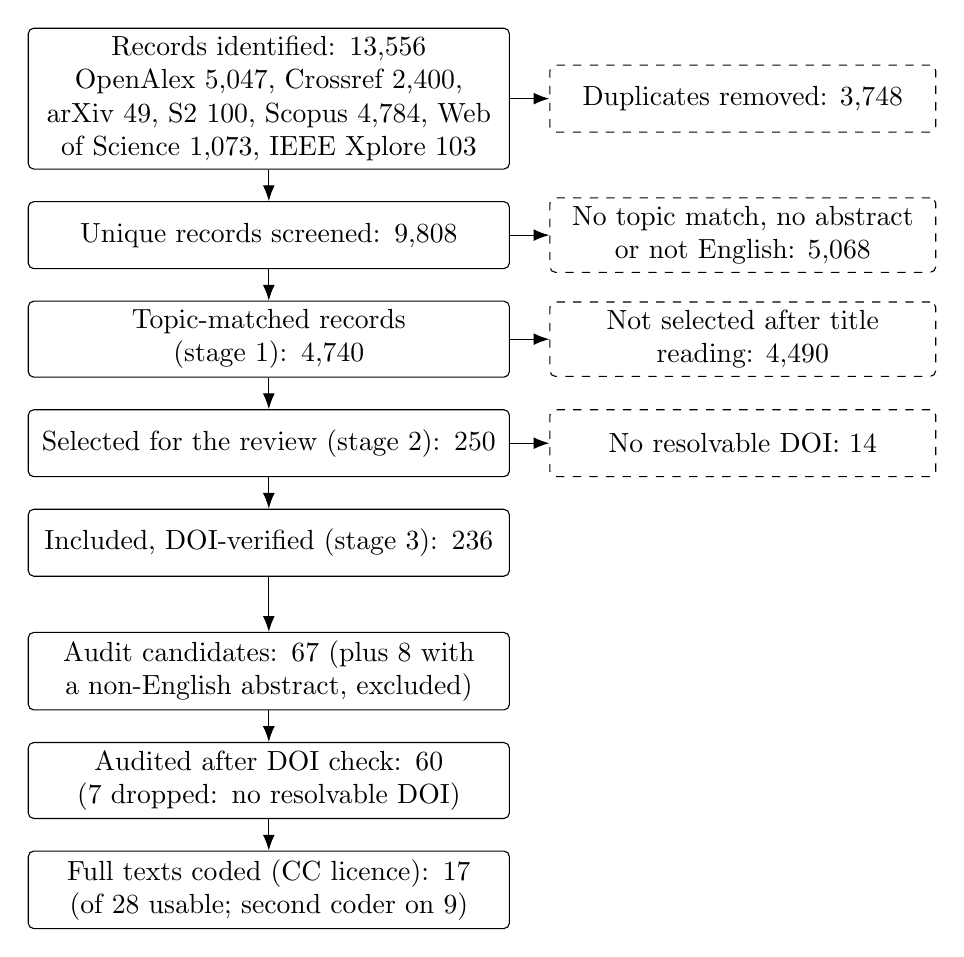
\begin{tikzpicture}[box/.style={draw,rounded corners=2pt,align=center,text width=5.9cm,minimum width=6.1cm,minimum height=0.85cm,inner sep=3pt},side/.style={draw,dashed,rounded corners=2pt,align=center,minimum width=4.9cm,minimum height=0.85cm,inner sep=3pt},arr/.style={-{Latex[length=2mm]}},node distance=0.4cm]
\node[box] (a) {Records identified: \totRetrieved{}\\\srcFlow{}};
\node[box,below=of a] (b) {Unique records screened: \unionUnique{}};
\node[box,below=of b] (c) {Topic-matched records (stage 1): \nStageOne{}};
\node[box,below=of c] (d) {Selected for the review (stage 2): \nSelected{}};
\node[box,below=of d] (e) {Included, DOI-verified (stage 3): \nVerified{}};
\node[side,right=0.5cm of a] (sa) {Duplicates removed: \dupRemoved{}};
\node[side,right=0.5cm of b] (sb) {No topic match, no abstract\\or not English: \exclStageOne{}};
\node[side,right=0.5cm of c] (sc) {Not selected after title\\reading: \exclStageTwo{}};
\node[side,right=0.5cm of d] (sd) {No resolvable DOI: \nDropped{}};
\foreach \i/\j in {a/b,b/c,c/d,d/e} \draw[arr] (\i) -- (\j);
\foreach \i/\j in {a/sa,b/sb,c/sc,d/sd} \draw[arr] (\i) -- (\j);
\node[box,below=0.7cm of e] (f) {Audit candidates: \nAuditCand{} (plus \nAuditLang{} with a non-English abstract, excluded)};
\node[box,below=of f] (g) {Audited after DOI check: \nAudit{}\\(\nAuditDropped{} dropped: no resolvable DOI)};
\node[box,below=of g] (h) {Full texts coded (CC licence): \ftN{}\\(of \ftAllN{} usable; second coder on \agN{})};
\draw[arr] (e) -- (f); \foreach \i/\j in {f/g,g/h} \draw[arr] (\i) -- (\j);
\end{tikzpicture}
\caption{Search and screening flow. All counts are generated from the screening files.}\label{fig:flow}
\end{figure}

\subsection{Audit coding}\label{sec:coding}
For the audit we kept geofence records whose title or opening abstract refers to attendance or presence monitoring, excluded reviews, and kept only abstracts written in English, because our rules are English patterns (\nAuditLang{} candidates were excluded for this reason, mostly Indonesian-language papers; they are real systems, so the audit describes English-abstract systems only). Fig.~\ref{fig:flow} shows how the audit set was reached.

\emph{Abstract level.} We coded the abstracts with a regular expression for each property (second factor, boundary shape, proxy or fraud wording, any number, privacy wording, LPWAN) and by hand for two properties that patterns cannot judge: whether the abstract reports a measurement of the geofence decision or the position error (as opposed to face-recognition accuracy, latency or usability scores), and whether it states that location error is handled or modelled.

\emph{Full text.} For the audited papers with a downloadable open-access version that carries a Creative Commons licence we coded seven yes/no questions (Table~\ref{tab:fulltext}), written down before coding and applied to keyword-in-context snippets from the full text. A property is coded present only if a snippet gives explicit evidence. We did not bypass paywalls or access controls, and we did not redistribute the texts.

\emph{Second coder.} A second coder, an AI model, coded \agNAll{} randomly chosen full-text papers from the same snippets without seeing our codes; \agN{} of them carry a Creative Commons licence and enter the agreement figures. We report agreement before adjudication, then resolved the one disagreement among them by rereading the source. One author (LHP) then read each of the \ftN{} full texts in full and checked every full-text code against the paper. The author saw the codes first, so this is a check and not an independent re-coding.

\subsection{Comparison group and reporting practice}
To test whether thin reporting is specific to geofencing, we applied the same abstract-level rules to every non-geofence attendance system in the corpus that is not a review (\nOthers{} records). Modality was assigned from the title, then from the opening abstract, using keywords (face, fingerprint or biometric, RFID, NFC or smart card, BLE or Bluetooth, QR, Wi-Fi). An accuracy figure was extracted from the abstract where a percentage of 50--100 appears next to the word ``accuracy''. These are reported figures on different data sets, so we use them to describe reporting practice, not to rank modalities.

\subsection{Use of AI tools}\label{sec:ai}
An AI assistant (Claude, Anthropic, used through Claude Code; the session log records the models \texttt{claude-sonnet-5-5} for nearly all responses and \texttt{claude-opus-5-5} for a few, between 3 and 12 November 2026) did four jobs. It wrote the search, screening and analysis scripts. It applied the coding rules to abstracts and to keyword-in-context snippets of full texts as the first coder, and, on a random sample of \agNAll{} papers, as a blind second coder. It drafted the text. And it formatted the manuscript. We used it because the corpus was too large to code by hand in the time we had and because the rules are mechanical enough to script. The assistant read publishers' abstracts and short keyword-in-context extracts of open-access full texts, not whole papers. In a first pass it read extracts of \ftAllN{} open-access papers; \ftLicCC{} of them carry a Creative Commons licence and \ftLicNone{} are free to read but record no Creative Commons licence (the recorded licence of every paper is listed in the supplementary files). PeerJ asks for permission from the copyright holders before copyrighted material is put into an AI tool, and we have not obtained it. The codes for the \ftLicNone{} papers without a Creative Commons licence are therefore not used in any table, figure or count in this article, and the full-text results rest on the \ftLicCC{} papers with a Creative Commons licence alone. The full prompts and session records are kept and can be given to the editor on request. The authors, not the assistant, are responsible for the content. \humanThreat{}

\subsection{Threats to validity}
Because no protocol was registered, we cannot show that the rules were fixed before the data were seen. Ranked retrieval caps what we see per query, and relevance in these indexes is loose, so the sample is not exhaustive; yearly counts reflect indexing and query design as well as publication volume. \srcThreat{} Abstract-level properties are lower bounds, and the full-text check covers only the \ftCcPct\% of audited papers (\ftN{} papers) whose open-access copy carries a Creative Commons licence, which may differ from the rest. Many audited papers come from small venues (Table~\ref{tab:venue}), and we did not assess venue quality. \humanThreat{} The 2026 count is for a partial year.

%--------------------------------------------------------------------
\section{Background}
\subsection{Geofence decisions and location error}
A circular geofence tests whether the great-circle distance between a fix and a centre is below a radius; the Haversine formula \cite{sinnott1984haversine} is the usual choice. A polygon fence uses a point-in-polygon test, for example ray casting or the winding number. Either test is applied to a measured position, not the true one. Smartphone GPS accuracy depends strongly on the environment \cite{zandbergen2009iphone,@11,schipperijn2014dynamic}, and a recent empirical study of smartphone GNSS for geofenced operation finds that the environment is the main driver of error, with large errors even outdoors next to buildings \cite{@1596}. In urban canyons the error can be reduced with 3D city models, for example by correcting pseudoranges \cite{@41}; such methods need building models and extra computation, and none of the \nAudit{} audited abstracts mentions shadow matching, 3D maps or map matching. Errors are also correlated in time: successive fixes tend to err in the same direction. A person standing near the boundary can therefore flip between inside and outside repeatedly (``flapping''). Section~\ref{sec:unc} returns to this.

\subsection{LoRa in brief}
LoRa is a chirp-spread-spectrum physical layer; LoRaWAN adds a MAC layer in which class-A devices transmit when they have data and listen afterwards. The ALOHA-like access makes capacity depend on the number of devices, the spreading factors in use, the number of channels and the capture effect \cite{augustin2016lora,@3,@4}. In India the 865--868~MHz band is open to short-range devices under a licence exemption \cite{dot865}; we cite the rule from secondary sources and have not checked the gazette text.

%--------------------------------------------------------------------
\section{A taxonomy of attendance and presence sensing}\label{sec:tax}
Table~\ref{tab:tech} organises the approaches we found by what counts as evidence of presence. The comparison is our qualitative synthesis from the cited works; it is not a measurement, and the limitation column mixes what papers report with what follows from the mechanism.

\begin{table}[tbp]\centering\footnotesize
\caption{Attendance and presence sensing approaches (qualitative synthesis by the authors; the works behind each row are cited in the paragraphs below).}\label{tab:tech}
{\setlength{\tabcolsep}{4pt}\begin{tabular}{@{}L{2.3cm}L{2.5cm}L{1.9cm}L{2.1cm}L{2.9cm}@{}}\toprule
Approach & Evidence of presence & User carries & Fixed infrastructure & Typical limitation \\ \midrule
RFID, NFC, smart card & Card or tag near a reader & Card, tag or phone & Reader at each entry & Cards can be shared; queue at the reader \\
BLE, Bluetooth & Phone near a beacon & Phone with app & Beacons per room & Phones can be shared; indoor radio varies \\
Fingerprint, iris, voice & Biometric match & Nothing & Scanner & Hardware cost; queues; hygiene \\
Face recognition & Face matched on camera or phone & Nothing or phone & Cameras and compute & Privacy; lighting; photo spoofing, hence liveness checks \\
QR code & Scan of a session code & Phone & Screen or print & Codes can be forwarded \\
GPS geofence on a phone (Section~\ref{sec:audit}) & Position inside a boundary & Phone with app & None beyond GNSS & Location error; mock locations; battery; privacy \\
GPS geofence on a LoRa node & Node position, sent over LPWAN & Wearable or card node & LoRa gateway(s) & Node cost; duty cycle; capacity; privacy \\
RFID plus LoRa & Card read, sent over LPWAN & Card & Reader node and gateway & As RFID, plus range \\ \bottomrule
\end{tabular}}
\end{table}

\paragraph{Credential-based} RFID, NFC and smart-card systems are the oldest and most numerous, from early RFID attendance designs \cite{@36,@86} to IoT versions with microcontrollers and cloud back ends \cite{@80,@210,@225,@287}. NFC has also been used, alone \cite{@167,@270} and in a comparison with RFID \cite{@250}. The presence evidence is possession, so a shared card defeats it.

\paragraph{Proximity radio} Bluetooth and BLE beacons tie a phone to a room \cite{@159,@165}, and BLE indoor positioning has been proposed for classroom attendance \cite{@209}. Indoor localisation in general is covered by a large survey \cite{@0}.

\paragraph{Biometrics and vision} Fingerprint \cite{@47,@168,@142} and face recognition \cite{@16,@33,@65,@71,@78} dominate the literature by volume. Vision systems have been extended to crowded classrooms with a phone camera \cite{@242}, to deep-learning pipelines \cite{@300} and to liveness detection \cite{@226}. The ethics of facial recognition and of surveillance in education is a recurring concern \cite{@21,@645}.

\paragraph{Code- and app-based} QR attendance \cite{@61} is cheap, but a systematic review of QR systems reports security measures such as randomised and dynamic codes combined with geofencing and device identifiers \cite{@1065}, which suggests the code alone is not trusted.

\paragraph{Location-based} Geofence attendance on phones is the subject of Section~\ref{sec:audit}. The LoRa-based attendance designs we found use cards, tags or NFC as the presence sensor and LoRa as the backhaul: a smart-card module for a large campus area evaluated by RSSI, SNR and packet loss \cite{@850}, an RFID and ESP32 design \cite{@1354}, an RFID and LoRa system tested to 133~m outdoors \cite{@1355}, a UTAUT adoption study of a LoRa attendance device with 40 respondents \cite{@1353}, and LoRa-based child-tracking and safety platforms that include attendance \cite{@851,@1000}. None of the abstracts mentions GPS or geofencing. LoRa geofencing exists elsewhere, for livestock, patients and wildlife \cite{@357,@1235,@1870,lopezescobar2025wildlife}, but we found no work that places a GPS geofence on a LoRa node to take attendance.

\subsection{Reporting practice across modalities}\label{sec:modality}
Table~\ref{tab:modality} counts the \nOthers{} non-geofence attendance systems in the corpus by modality and shows how often their abstracts report an accuracy figure, a sample size, spoofing concerns and privacy. Face recognition dominates (\modFace{} records), followed by fingerprint, iris or voice (\modBio{}), RFID (\modRfid{}), QR (\modQr{}), NFC or smart card (\modNfc{}), BLE (\modBle{}) and Wi-Fi (\modWifi{}); \modUnspec{} do not name a modality. Reporting is thin everywhere. Even for face recognition, only \modAccPctFace\% of abstracts give an accuracy percentage, with a median of \modAccMedFace\%; for RFID the share is \modAccPctRfid\%. Sample sizes are rarer still. Reported accuracies cluster at the top of the scale and come from different data sets, so they should not be compared across rows.

\begin{table}[tbp]\centering\footnotesize
\caption{Reporting practice by sensing modality among \nOthers{} non-geofence attendance systems in the corpus (abstract level). ``Accuracy'' = abstracts giving an accuracy percentage; the median and range are of those values. These are reported figures on different data sets and are \emph{not} comparable performance rankings.}\label{tab:modality}
\resizebox{\linewidth}{!}{\begin{tabular}{@{}lrrrrrr@{}}\toprule Modality & Systems & Report accuracy & Median (range) \% & Report sample size & Mention spoofing & Mention privacy \\ \midrule
Face recognition & 922 & 207 (22\%) & 95.7 (50--100) & 65 (7\%) & 274 (30\%) & 66 (7\%) \\
Fingerprint, iris, voice & 255 & 31 (12\%) & 95.6 (69--100) & 15 (6\%) & 84 (33\%) & 11 (4\%) \\
RFID & 171 & 8 (5\%) & 93.5 (80--97) & 2 (1\%) & 34 (20\%) & 5 (3\%) \\
NFC, smart card & 39 & 1 (3\%) & n$<$5 & 2 (5\%) & 13 (33\%) & 1 (3\%) \\
BLE, Bluetooth & 47 & 0 (0\%) & -- & 4 (9\%) & 10 (21\%) & 4 (9\%) \\
QR code & 120 & 4 (3\%) & n$<$5 & 11 (9\%) & 32 (27\%) & 6 (5\%) \\
Wi-Fi & 14 & 1 (7\%) & n$<$5 & 1 (7\%) & 2 (14\%) & 0 (0\%) \\
Unspecified & 758 & 26 (3\%) & 97.5 (53--100) & 63 (8\%) & 97 (13\%) & 12 (2\%) \\
\bottomrule\end{tabular}}\end{table}


\subsection{Geofencing beyond attendance}\label{sec:domain}
Geofencing is older and wider than attendance. Records outside attendance cover COVID-19 containment zones and quarantine monitoring \cite{@394,@753,@731}, livestock, wildlife and farming \cite{@95,@349,@1235,@1870}, drone airspace \cite{@185}, fleet tracking \cite{@701}, geofenced autonomous-vehicle services \cite{@336}, and location-based content in museums \cite{@307,@604}, with reviews in population health and behavioural research \cite{tobin2023geofencing,shevchenko2024geofencing}. Table~\ref{tab:domain} classifies the \nGeoAll{} geofence-titled records in the corpus. Attendance and workforce records are the largest group (\domAtt{}, \domPctAtt\%), ahead of marketing, tourism and location services (\domMkt{}), transport and logistics (\domVeh{}), health and care (\domHealth{}) and livestock and wildlife (\domLive{}). LoRa or LPWAN appears in only \domLoraTotal{} of the \nGeoAll{} records, \domLoraLive{} of them in livestock and wildlife. The breadth matters for this survey in two ways: the boundary-error question is not special to classrooms, and decision logic developed for one domain should transfer to the others.

\begin{table}[tbp]\centering\footnotesize
\caption{Application domains of the \nGeoAll{} geofence-titled records in the corpus (title and abstract rules, first match wins). Shares are of records in the row; abstract-level.}\label{tab:domain}
\resizebox{\linewidth}{!}{\begin{tabular}{@{}lrrrrr@{}}\toprule Domain & Records & Share & Mention LoRa/LPWAN & Mention energy & Mention location error or uncertainty \\ \midrule
Attendance, presence, workforce & 76 & 21\% & 0 & 2 & 5 \\
Health, COVID-19, elderly care & 36 & 10\% & 1 & 9 & 1 \\
Livestock, wildlife, farming & 27 & 8\% & 4 & 4 & 2 \\
Aviation, drones, UAV & 38 & 11\% & 0 & 0 & 11 \\
Vehicles, transport, logistics & 43 & 12\% & 1 & 5 & 4 \\
Marketing, tourism, location services & 58 & 16\% & 2 & 13 & 3 \\
Safety, security, access control & 39 & 11\% & 3 & 7 & 2 \\
Other or unclear & 41 & 11\% & 1 & 5 & 2 \\
\bottomrule\end{tabular}}\end{table}


%--------------------------------------------------------------------
\section{Geofence attendance systems: an evidence audit}\label{sec:audit}
\subsection{Growth and design patterns}
Of the \nAudit{} systems, \aEarly{} date from 2022 or earlier, \aYtwentythree{} from 2023, \aYtwentyfour{} from 2024, \aYtwentyfive{} from 2025 and \aYtwentysix{} from 2026 so far (Fig.~\ref{fig:year}); \aRecent{} (\pRecent\%) are from the last two years. The pattern most likely reflects both real growth and the indexing of small venues, and we cannot separate the two.

\begin{figure}[t]\centering
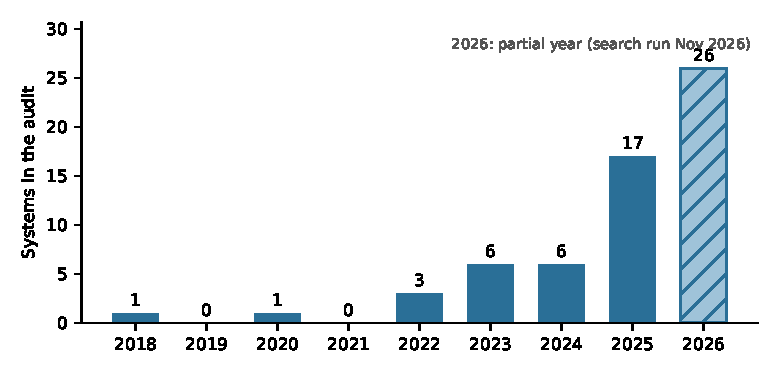
\includegraphics[width=0.62\linewidth]{gen/fig_year.pdf}
\caption{Geofence attendance systems in the audit, by year (\nAudit{} systems). The hatched bar is a partial year.}\label{fig:year}
\end{figure}

Table~\ref{tab:audit} lists the audited properties. Most systems treat the geofence as one check among several: \aSecond{} (\pSecond\%) add a second factor, most often face recognition (\aFace), another biometric (\aBio), QR codes (\aQr) or RFID, NFC or BLE (\aRfid). Where the boundary shape appears in the abstract, circles are more common (\aCircle) than polygons or boxes (\aPoly). A few add rules on top of the geofence: attendance is credited only after 80\% of the class duration spent inside \cite{@1253}, or when more than 90\% of the time is spent inside \cite{@538}. One design builds a polygon from users' geotags and checks it against a static campus polygon \cite{@1247}.

\begin{table}[tbp]\centering\small
\caption{Abstract-level audit of \nAudit{} geofence-based attendance and presence systems (counts overlap). Coding rules are in Section~\ref{sec:method}.}\label{tab:audit}
\begin{tabular}{@{}L{0.70\linewidth}rr@{}}\toprule
Property found in the abstract & Systems & Share \\ \midrule
Adds a second factor (face, biometric, QR, RFID/NFC/BLE, device ID) & 45 & 75\% \\
\quad face recognition or liveness & 28 & 47\% \\
\quad fingerprint, voice, iris or generic biometric & 21 & 35\% \\
\quad QR code & 14 & 23\% \\
\quad RFID, NFC or BLE & 8 & 13\% \\
Mentions proxy attendance, fraud or spoofing & 28 & 47\% \\
Boundary stated as circle (Haversine or radius) & 14 & 23\% \\
Boundary stated as polygon or box & 4 & 7\% \\
Reports any number (accuracy, latency, usability, sample size) & 23 & 38\% \\
\quad of which measures the geofence decision or position error & 6 & 10\% \\
States that location error or uncertainty is handled & 4 & 7\% \\
Mentions privacy or data protection & 3 & 5\% \\
Uses LoRa or another LPWAN & 0 & 0\% \\
\bottomrule\end{tabular}\end{table}


\subsection{What the abstracts report}
Only \aQuant{} of \nAudit{} abstracts (\pQuant\%) report any number. Most of these measure something other than the geofence: face-recognition accuracy, response time, a usability score or a questionnaire. \aMetric{} (\pMetric\%) report a measurement of the geofence decision or the position error:
\begin{itemize}
\item A teacher-presence application reports 100\% accuracy over 30 test runs \cite{mughni2023teacher}.
\item A face-and-geofence system reports 100\% location validation on five test coordinates, and 90\% accuracy over 30 combined location-and-face scenarios \cite{@1242}.
\item A hostel system reports 97.2\% geofencing accuracy with fifty student accounts \cite{@1992}.
\item A police-office deployment reports geofencing accuracy of 92.18\% in open areas, falling to 71.33\% in urban environments \cite{@992}. It is the only abstract in the audit that reports accuracy by environment.
\item A nurse working-hours study reports a positioning error of 1.4--3.7~m and a delay of 4.45--15.30~s when the user's position switches, depending on the device \cite{@1280}.
\item A session-bound attendance protocol simulates false acceptance and rejection under three location-error models over 30 seeds \cite{@1249}. At 15~m reported accuracy a fixed-radius rule gives 4.15\% false acceptance and 3.70\% false rejection; weighting the rule by reported uncertainty removes false acceptance but raises false rejection to 20.30\%.
\end{itemize}
The last item is the only audited abstract that quantifies the trade-off between letting the wrong person in and keeping the right person out. The same abstract reports that a forwarded token paired with fabricated inside-geofence coordinates was accepted \cite{@1249}, which is the only location-spoofing outcome in the audit.

\subsection{Location error, spoofing, privacy and scale}
\aLocerr{} abstracts state that location error is handled or modelled \cite{@1244,@1247,@1249,@1260}: dynamic geofencing that adapts to location errors, a distance tolerance, an uncertainty weight, and a fallback when location is unavailable or inaccurate. \aSpoof{} (\pSpoof\%) mention proxy attendance, fraud or spoofing as a motivation, but a keyword scan for adversarial outcomes finds only three abstracts that report one. Two test the face factor, with a false accept rate of 80.0\% at a face library's default threshold \cite{@1240} and screen-replay attacks scored by a liveness model \cite{@1306}; one tests the location factor \cite{@1249}. Only \aPriv{} abstracts mention privacy or data protection, although every system collects a person's position over time. No audited system uses LoRa or any LPWAN, and none reports energy measurements or capacity in its abstract.

\subsection{Is thin reporting specific to geofencing?}\label{sec:compare}
Table~\ref{tab:compare} applies the same abstract-level rules to \nOthersRecent{} other attendance systems from 2018 onward. Reporting is thin there too: \cmpOacc\% give an accuracy figure and \cmpOsample\% a sample size in the abstract, against \cmpGacc\% and \cmpGsample\% for the geofence systems. Geofence systems mention spoofing, proxy attendance or fraud more often (\cmpGspoof\% against \cmpOspoof\%) and mention privacy about as rarely (\cmpGpriv\% against \cmpOpriv\%). We therefore read the thin evidence as a habit of the attendance literature, not a failing of geofencing in particular. The audited papers are also concentrated in small venues: Table~\ref{tab:venue} splits them by venue type, but only \nCore{} of \nAudit{} are in OpenAlex core sources, \nOA{} are open access, and the counts per group are small. What is specific to geofencing is the property the abstracts rarely mention: how the boundary decision copes with position error, and how the location factor withstands manipulation.

\begin{table}[tbp]\centering\small
\caption{Geofence attendance systems (\nAudit{}) compared with other attendance systems from 2018 onward (2039), by the same abstract-level rules. Shares are percentages of systems.}\label{tab:compare}
\begin{tabular}{@{}lrr@{}}\toprule Property in the abstract & Geofence & Other \\ \midrule
Reports an accuracy percentage & 13 & 13 \\
Reports a sample size (users, images, trials) & 13 & 7 \\
Mentions spoofing, proxy or fraud & 45 & 26 \\
Mentions privacy or data protection & 5 & 5 \\
\bottomrule\end{tabular}\end{table}

\begin{table}[tbp]\centering\small
\caption{Venue type of the audited systems (OpenAlex source metadata) and the share that report any number or a geofence-decision measurement.}\label{tab:venue}
\begin{tabular}{@{}lrL{2.2cm}L{2.6cm}@{}}\toprule Group & Systems & Report any number & Geofence measurement \\ \midrule
OpenAlex core source & 6 & 4 & 1 \\
Other journal & 37 & 12 & 3 \\
Conference (not core) & 11 & 3 & 2 \\
Repository (Zenodo, arXiv) & 6 & 4 & 0 \\
\bottomrule\end{tabular}\end{table}


\subsection{Full-text check}\label{sec:fulltext}
Abstracts understate what papers do, so we also coded the full texts of the audited systems whose open-access copy carries a Creative Commons licence. Of \ftTried{} audited papers, full text was usable for \ftAllN{} (\ftPct\%); \ftNoOA{} are not open access, \ftShort{} resolved only to a landing page or a short page, and \ftErr{} failed to download. Of the \ftAllN{} usable texts, \ftN{} (\ftCcPct\% of the audited papers) carry a Creative Commons licence and are the basis of Table~\ref{tab:fulltext}; the other \ftLicNone{} are free to read but record no such licence and are left out (Section~\ref{sec:ai}). A blind AI second coder agreed with the first on \agPct\% of \agJ{} judgements over \agN{} of these papers (Cohen's $\kappa=\agKappa$; $\kappa$ is undefined for the three questions where neither coder found a yes). The one disagreement was resolved by rereading: a forwarded-token attack that the paper's abstract reports but the snippets did not show (kept as yes).\humanSentence{} The author check of all \ftN{} papers is described in Section~\ref{sec:coding}. The check changed none of the \ftCodes{} full-text codes.

Reading the full text changes the picture only a little. Location error is handled or analysed in \ftQone{} of \ftN{} papers, against \ftAbsQone{} by abstract; the geofence decision is measured in \ftQtwo{} (\ftAbsQtwo{} by abstract); \ftQthree{} report an adversarial test; and the fence itself (a radius or polygon) is stated in \ftQseven{}. None states a location sampling policy, reports energy or discusses privacy beyond a passing word. Abstract-level coding therefore undercounts, mainly for location-error handling, but what abstracts omit is mostly absent from the papers too. With \ftN{} papers the counts are small, and the \ftLicNone{} papers left out for copyright reasons may differ.

\begin{table}[tbp]\centering\small
\caption{Full-text check of the \ftN{} audited papers whose open-access copy carries a Creative Commons licence: papers with the property, by full-text coding and by abstract-level coding of the same papers (``--'' = not coded at abstract level). Full-text codes are adjudicated; see Section~\ref{sec:fulltext}.}\label{tab:fulltext}
\begin{tabular}{@{}lrr@{}}\toprule Property & Full text & Abstract only \\ \midrule
Location error handled or analysed & 2 & 1 \\
Geofence decision or position error measured & 3 & 3 \\
Adversarial test with an outcome & 2 & 2 \\
Location sampling policy stated & 0 & -- \\
Energy measured or modelled & 0 & -- \\
Privacy or data protection discussed & 0 & 1 \\
Fence parameters stated & 5 & -- \\
\bottomrule\end{tabular}\end{table}


%--------------------------------------------------------------------
\section{Boundary decisions under location uncertainty}\label{sec:unc}
Outside attendance, the geofencing literature treats uncertainty more directly. Reliability of proactive location services depends on the geofence configuration, and a web service has been proposed that estimates how reliable a service is for a given fence \cite{@751}. When fixes are sparse because of weak signal, privacy or energy saving, an entry can go unnoticed, and short-term location prediction has been used to compute the probability of entering a fence \cite{@990}. Cellular signal comparison offers a low-energy and privacy-preserving way to detect arrival at a known place \cite{@521}. Fence geometry has been designed from data \cite{@754,@1018,@1019}, UWB positioning has been examined for geofencing in a factory safety case \cite{@976} and with a one-class classifier \cite{@1457}, and an outsourced scheme uses Bloom filters to keep locations private \cite{@659}. Learning-based methods have also been proposed: neural networks that decide whether a point lies inside a fence \cite{@857} and meta-reinforcement learning for tracking \cite{@902}.

Decision logic can be arranged on a ladder of increasing protection against error:
\begin{enumerate}
\item a single-fix radius test, which the audit shows is the usual choice;
\item a polygon test, which matches the shape of campuses \cite{@1247};
\item a hysteresis band, which requires the measured distance to pass the boundary by a margin;
\item $k$-of-$n$ confirmation or a dwell time, as in \cite{@1253,@538};
\item sequential evidence accumulation, a CUSUM-style detector \cite{page1954cusum};
\item uncertainty-weighted acceptance \cite{@1249}; and
\item prediction across gaps in the fixes \cite{@990}.
\end{enumerate}
Steps 3 to 5 are standard in signal detection, but we found no attendance paper that analyses them, and the audit finds dwell rules without a justification for the dwell length. The companion study in Section~\ref{sec:case} measures steps 1, 3, 4 and 5 on real tracks.

%--------------------------------------------------------------------
\section{Energy and sampling}\label{sec:energy}
Taking fixes is the dominant cost of a GPS tracker, and a long line of work reduces it by duty cycling and by using cheaper sensors to bound the uncertainty. Examples include adaptive GPS duty cycling with radio ranging \cite{jurdak2010adaptive}, EnTracked \cite{kjaergaard2009entracked}, rate-adaptive positioning \cite{paek2010raps}, EnLoc \cite{constandache2009enloc}, energy--accuracy trade-offs for continuous location \cite{lin2010aloc} and DuctiLoc \cite{katsikouli2023ductiloc}. Studies of smartphone applications examine how GPS signal strength affects power use and how to cut the energy of GPS-based location sensing \cite{@115,@152}. For LoRa nodes, GPS-free localisation is possible from gateway measurements \cite{fargas2017gpsfree} and has been surveyed \cite{@465,@466,@67,@3255}, and public Sigfox and LoRaWAN fingerprint data sets cover large urban and rural areas \cite{@34}, but RSSI-based approaches are coarse, and a geofence at campus scale needs metre-level decisions. LoRa trackers that keep the GPS off until needed report battery savings: a cattle geofence system reports 93\% geofencing accuracy and about 35\% battery saving from conditional GPS operation \cite{@1235}, and energy-efficient LoRa GPS trackers have also been built for dementia patients and for wildlife \cite{@206,lopezescobar2025wildlife}. Energy models for LoRa nodes \cite{bouguera2018energy,casals2017energy} and for LPWAN technologies \cite{@55} are available, but none of the full texts we coded reports energy.

One factor is easy to miss. Energy estimates need a time per fix. A hot start with retained ephemeris takes a second or two, while a cold start can take tens of seconds, and adaptive sampling loses most of its advantage if every fix is a cold start. Section~\ref{sec:case} gives numbers.

%--------------------------------------------------------------------
\section{LPWAN scalability and synchronised arrivals}\label{sec:lpwan}
The LoRa capacity literature is large. Surveys cover the technology and its applications \cite{@3,@3162}, compare it with other LPWAN technologies \cite{@1} and set out application requirements \cite{@13}; others treat scalable LoRaWAN for massive IoT \cite{@4}, adaptive data rate \cite{@22} and energy efficiency \cite{@191,@311}. One experimental study tests the manufacturer's claims \cite{@6}. Analytical and simulated studies ask whether LoRa scales \cite{bor2016scale,georgiou2017scale,adelantado2017limits,@10}, how imperfect orthogonality changes the answer \cite{mahmood2019scalability,@3165}, what frame collisions look like \cite{rahmadhani2018collide} and what smart-metering deployments can reach \cite{varsier2017capacity}. Measurement studies report coverage and scalability \cite{@3166,@3168} and reliability on a testbed \cite{@14}; power and spreading-factor control address the near--far effect \cite{@20}, and the effect of bidirectional traffic has been examined \cite{@29}. Scheduling \cite{@15,@44}, a time-slotted design \cite{@37}, a slotted-ALOHA overlay \cite{@24} and alternative random-access protocols \cite{@51} raise capacity at the cost of synchronisation or protocol changes.

These analyses mostly assume independent traffic. Attendance traffic is not independent. Presence changes cluster at timetable boundaries, so the load a gateway sees in the minute after a lecture ends is a multiple of its daily mean. The LoRa attendance papers we found report coverage and link quality (RSSI, SNR, packet loss, range) \cite{@850,@1355}; none of the abstracts evaluates capacity under synchronised arrivals. A lecture hall is an indoor setting, and indoor LoRaWAN deployments have been examined in a case study \cite{@25}. The LoRa geofencing papers report range and latency, such as up to 1~km at an RSSI of $-105$~dB for elephant monitoring \cite{@1870}, or a mesh design for remote communities \cite{@357}. Section~\ref{sec:case} quantifies the burst effect on real class-change data.

%--------------------------------------------------------------------
\section{People in the loop: privacy, regulation and security}\label{sec:priv}
An attendance system is a cyber-physical system with a person in the loop: the person carries the sensor, is judged by the decision, and bears the cost of a wrong one. This section looks at the system from that side.

\subsection{Location data about people}
A geofence attendance system records where a person is, and when, for as long as the log is kept. The location-privacy literature is large \cite{@75,krumm2009privacy,beresford2003location}, including anonymity-based schemes \cite{@43} and a comparative overview of methods \cite{@312}. Obfuscation and differential-privacy methods exist for location-based services \cite{@2061,@2093}. They blur the position, and an attendance decision needs an accurate position near the boundary, so noise large enough to hide a person is likely to flip the decision; this is our reading, not a result of the cited papers. India's Digital Personal Data Protection Act 2023 \cite{dpdp2023} has been evaluated for privacy rights and state surveillance \cite{@1641}, and student data raise further concerns \cite{@8,@645}. In the \ftN{} full texts we coded, none discusses privacy beyond a passing word. A keyword scan of the \hfN{} audited abstracts finds \hfConsent{} that mention consent or an opt-in or opt-out choice.

\subsection{Legal duties that shape the design}
This is a summary of duties that bear on design, not legal advice, and the texts should be read in full. Under the GDPR \cite{gdpr2016}, personal data must be collected for a stated purpose, limited to what is needed and kept no longer than necessary (Art.~5(1)). Consent is unlikely to be freely given where the person and the controller stand in a clear imbalance of power (Recital~43), which describes an institution and its students or staff. The effect of the GDPR on location data in particular is discussed in \cite{@278}. India's Digital Personal Data Protection Act 2023 \cite{dpdp2023} likewise ties processing to consent or to listed legitimate uses, requires notice to the person, lets the person withdraw consent, and requires erasure once the purpose is served. Section~9 adds two rules for children (persons under 18): verifiable consent of a parent or guardian, and a bar on tracking or behavioural monitoring of children. Rules made under the Act can exempt classes of data fiduciary from both, and the Digital Personal Data Protection Rules 2025 do so for educational institutions: the Fourth Schedule (Part A, entry 3, referred to from rule 12) lifts sections 9(1) and 9(3) only for tracking and behavioural monitoring done for the institution's educational activities or in the interests of the safety of children enrolled with it \cite{dpdp2025rules}. A continuous location log of a school pupil sits close to the monitoring that section~9 restricts, so an attendance system for minors needs a legal reading before deployment. We do not settle which systems are exempt.

Two design consequences follow from these principles, not from the audit. An inside-or-outside decision needs less data than a position track, so evaluating the fence on the phone or tracker and sending only boundary events meets the minimisation principle more easily than uploading raw fixes. And a retention period has to be chosen and stated, because a log kept for ever serves no attendance purpose.

\subsection{Where the person is the weak point}
\emph{The location factor attests a phone, not a person.} A friend who carries two phones, a mock-location app or a shared login defeats it. In the audit, a keyword scan finds \hfDevBind{} of \hfN{} abstracts that mention a device identifier such as an IMEI or device ID, and \ftQthree{} of \ftN{} full texts report an attack test.

\emph{Errors fall on people unequally.} A false absence can cost a student exam eligibility, while a false presence helps someone who cheats. Papers report an accuracy figure but not who is misclassified or what happens next. A plain radius test produced 0.455 spurious events per track-hour in the companion study (Section~\ref{sec:case}), and a spurious exit event can turn a present person into an absent one unless the rule or a human corrects it. We did not code whether the audited papers describe an appeal or override route, and a keyword scan is too coarse to report a number.

\emph{Consent is weak in captive populations.} Qualitative work on workplace monitoring reports how workers understand and respond to surveillance technologies \cite{@332}. If students cannot refuse in practice, the system needs an equal alternative for people who decline or have no suitable phone, and the cost of running two systems should be counted. Face recognition raises privacy and bias concerns of its own \cite{@21,@645}; a geofence avoids biometrics but not inequality of devices, since older phones and denied location permissions give worse fixes or none.

Table~\ref{tab:human} turns these points into design requirements and states what the audit can say about each.

\begin{table}[tbp]\centering\footnotesize
\caption{Design requirements for presence sensing with a person in the loop, the basis of each, and what the audit evidence shows. ``Not coded'' means we did not code the property.}\label{tab:human}
\begin{tabular}{@{}L{4.4cm}L{3.5cm}L{4.4cm}@{}}\toprule
Requirement & Basis & Audit evidence \\ \midrule
Evaluate the fence on the device and send only the event & GDPR Art.~5(1); purpose limits in the DPDP Act & Not coded; privacy is discussed in \ftQsix{} of \ftN{} full texts \\
State a retention period and erase when the purpose ends & GDPR Art.~5(1); DPDP Act erasure duty & Not coded \\
Offer an equal alternative to people who decline or cannot use a phone & GDPR Recital~43; withdrawal of consent under the DPDP Act & Consent, opt-in or opt-out in \hfConsent{} of \hfN{} abstracts \\
Bind the record to a device and test relay, mock-location and shared-device attacks & Security (Section~\ref{sec:sec}) & Device identifier mentioned in \hfDevBind{} of \hfN{} abstracts; an attack test in \ftQthree{} of \ftN{} full texts \\
Give a route to correct a wrong record & A false absence harms the person & Not coded \\
Check the age rules before tracking pupils under 18 & DPDP Act section~9 & Not coded \\ \bottomrule
\end{tabular}
\end{table}

\subsection{Attacks on location and radio}\label{sec:sec}

Security has two sides. Location can be forged: the requirements for a successful GPS spoofing attack are well studied \cite{tippenhauer2011spoofing,psiaki2016gnss}, spoofing in networks of drones has been reviewed systematically \cite{@128}, and detection methods include dual-receiver correlation of encrypted signals \cite{@27}, multi-receiver detection \cite{@195}, a single-antenna correlator technique \cite{@114} and checks on the outputs of commercial receivers \cite{@223}. A software-level attack, such as a mock location on a phone, needs no radio hardware at all and is what the audited systems most often mention. The radio can also be attacked: LoRaWAN has known weaknesses in activation, key handling and the join procedure \cite{@54,@17,@62,@82,@237,@313}. Timing is a less discussed leak. Even with encrypted payloads, packet times reveal when someone crosses a boundary, and our companion study measures this (Section~\ref{sec:case}).

%--------------------------------------------------------------------
\section{Case study: what the neglected issues cost}\label{sec:case}
To show that the gaps in Sections~\ref{sec:audit}--\ref{sec:lpwan} matter, we summarise a companion simulation study (Dhanisha S, Lakshmi Harika P, Adesh Kanna P and Ananyaa S, unpublished data, 2026). It is a simulation and a replay of public data, with no new hardware measurements, and it is included to give orders of magnitude, not as a contribution of this survey. It uses a 10-byte LoRa packet with a counter and a truncated HMAC, a hysteresis-plus-dwell detector and boundary-proximity adaptive sampling. Real position errors come from the GeoLife GPS trajectories \cite{zheng2009geolife} and real crossing times from the StudentLife dataset \cite{wang2014studentlife}. The simulator, and a script that checks every number in Table~\ref{tab:case} against its result files, are in the repository \todo{URL to be added}.

\begin{table}[tbp]\centering\footnotesize
\caption{Companion-study results for the issues raised by the audit (simulation and replay of public data).}\label{tab:case}
\begin{tabular}{@{}L{3.2cm}L{9.4cm}@{}}\toprule
Issue (section) & Result \\ \midrule
Flapping at the boundary (\ref{sec:unc}) & On 311 real pedestrian segments (255 track-hours), a plain radius test gave 0.455 spurious events per track-hour (95\% interval 0.330--0.627, resampling users). A hysteresis detector with adaptive sampling gave 0.027 (0.011--0.049), about 94\% fewer, while missing 1.6\% of proxy-truth transitions at a $\pm$10~m tolerance. Mean detection delay was 29.4~s. \\
Is a better detector available? (\ref{sec:unc}) & An evidence-accumulation detector improved on the best hysteresis settings by only 1--4~s (3--14\%) at equal false-toggle rates. The choice of band width mattered more than the detector family. \\
Sampling and fix time (\ref{sec:energy}) & On the real tracks, adaptive sampling cut fixes from 720 to 144 per hour ($5.0\times$) and the modelled battery life rose from 1.8 to 8.8 days, assuming a 2~s fix. In the simulated scenario, battery life fell from 14.8 days with 2~s fixes to 2.0 days with 15~s fixes. \\
Synchronised arrivals (\ref{sec:lpwan}) & On real student-day crossing times, a single gateway at 95\% event delivery carried about 6{,}700 students, against 7{,}900 for the same events spread uniformly: ordinary class changes cost about 15\%. If every student crosses at the same second, 240~s of random delay supports about 1{,}000 students, and one blind repetition about 2{,}100. \\
Timing leakage (\ref{sec:priv}) & A passive eavesdropper estimated crossing times to a median 4~s (97\% within a minute) without random delay, and to 60~s (50\% within a minute) with 240~s of delay. Delay blurs timing; it does not hide it. \\ \bottomrule
\end{tabular}
\end{table}

Three points follow. First, the false-event rate of the plain test is large enough to matter for a daily roll call, so the first rung of the decision ladder is not safe to use alone. Second, the more elaborate detector is not the main lever; the margin and the sampling policy are. Third, burst effects on capacity are real but moderate for ordinary timetables, and severe only for hard synchronisation such as a bell or a bus departure. The companion study's own limitation applies here: energy and radio figures are modelled, not measured, and the burst study uses one university's timing. We cite it to size the problems, not to prove the solutions.

%--------------------------------------------------------------------
\section{A minimum reporting checklist}\label{sec:checklist}
Sections~\ref{sec:audit}--\ref{sec:priv} show the same pattern: the properties that decide whether a presence system can be trusted are the ones papers leave out. We turn the seven full-text questions of Section~\ref{sec:fulltext} into a checklist of items that an attendance or presence-sensing paper should report (Table~\ref{tab:checklist}). The items were chosen because each decides something a reader needs. R1 and R2 say whether the decision is right, R3 whether it can be gamed, R4 and R5 whether it can run on a battery, R6 whether it can run lawfully, and R7 whether anyone can repeat it. R2, R3 and R6 apply to every modality, so an RFID, QR or face system can be scored on them too.

\begin{table}[tbp]\centering\footnotesize
\caption{Proposed minimum reporting checklist for presence-sensing papers, with the number of the \ftN{} full-text-coded geofence attendance papers (Creative Commons licence) that meet each item. Items R1--R7 are the codebook questions of Section~\ref{sec:fulltext}; no item was scored as not applicable, so counts for R4, R5 and R7 are low for papers where an item arguably does not apply. The codebook definitions of R1 and R6 are looser than the wording here (``handled or analysed'', ``discussed''), so the counts for those two overstate compliance.}\label{tab:checklist}
\begin{tabular}{@{}lL{7.4cm}L{2.2cm}r@{}}\toprule Item & Report & Applies to & Met \\ \midrule
R1 & Position error of the sensing method under the test conditions (for example median and 95th percentile), and how the decision rule copes with it. & Location-based & 2 of \ftN{} \\
R2 & Error of the presence decision itself against ground truth: false entries, false exits, missed events, delay. & All modalities & 3 of \ftN{} \\
R3 & At least one attack on the presence factor (mock location, forwarded or relayed token, photo or replay, shared device) and its outcome. & All modalities & 2 of \ftN{} \\
R4 & When and how often the person or tag is sampled, and what triggers a sample. & Location-based & 0 of \ftN{} \\
R5 & Energy per day or battery life, measured or modelled with the fix or read time stated. & Battery-powered & 0 of \ftN{} \\
R6 & Personal data collected, retention period, legal basis or consent route, and who can read the log. & All modalities & 0 of \ftN{} \\
R7 & Fence shape and size, thresholds, dwell or confirmation rule, and the values used in the test. & Geofence & 5 of \ftN{} \\
\bottomrule\end{tabular}\end{table}


\begin{figure}[tbp]\centering
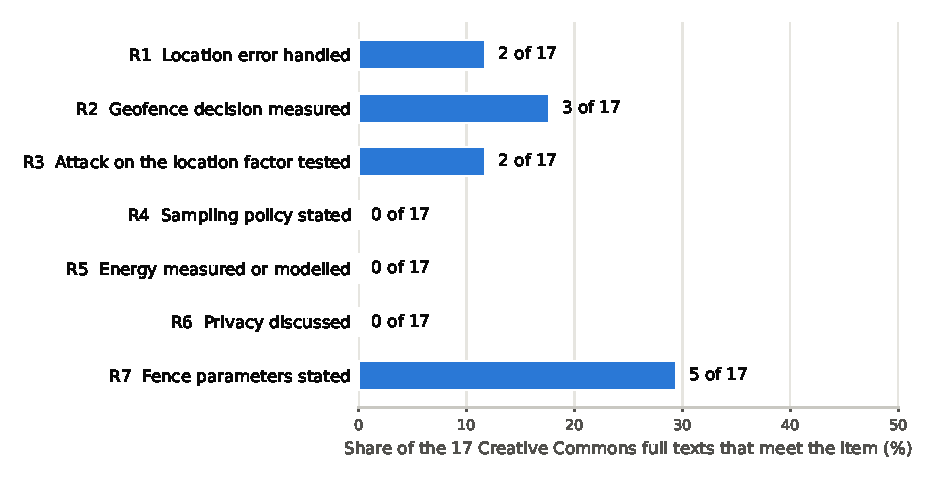
\includegraphics[width=0.82\linewidth]{gen/fig_reporting.pdf}
\caption{Share of the \ftN{} full-text-coded papers (Creative Commons licence) that meet each reporting item R1--R7. Labels give papers met of papers coded.}\label{fig:reporting}
\end{figure}

Applied to the \ftN{} full texts, \ftScoreZero{} papers meet none of the seven items, \ftScoreOne{} meet one, \ftScoreTwo{} meet two and \ftScoreThree{} meet three; none meets more (Fig.~\ref{fig:reporting}). The papers with three are \ftBestCites{}. This is a description of reporting, not a ranking of quality: several papers are short application descriptions that never set out to evaluate anything. A trial size and a source of ground truth belong on the list as well, but we did not code them in the full texts, so Table~\ref{tab:checklist} omits them; at abstract level a sample size appears in \cmpGsample\% of the geofence abstracts and \cmpOsample\% of the other attendance abstracts.

We suggest that authors report R1--R7 as ``yes'', ``no'' or ``not applicable'', each with a section number, in a short table. The checklist has limits. It was derived from the same papers it scores, so the counts are a description and not a validation. Nobody outside the author team has tested the wording, no item is weighted, and an item can be met with weak evidence. We publish the codebook and the coding sheets so that others can refine the items.

%--------------------------------------------------------------------
\section{Open challenges and research agenda}\label{sec:agenda}
\begin{enumerate}
\item \textbf{A shared benchmark.} The audit finds no common test. A benchmark should supply ground-truth trajectories with labelled crossings, realistic error models and agreed metrics: false events per hour, detection delay, missed crossings and roll-call accuracy. GeoLife and StudentLife are starting points \cite{zheng2009geolife,wang2014studentlife}, but neither was built for attendance.
\item \textbf{Report and use location uncertainty.} Phones expose a reported accuracy. The only abstract that uses it shows a large false-rejection price for the safety gained \cite{@1249}. Decision rules that trade the two errors explicitly, and are validated on real tracks, are missing.
\item \textbf{Adversarial evaluation of the location factor.} Mock locations, relayed or forwarded tokens, shared devices and replayed packets should be tested and the outcomes reported, as one audited paper does for a forwarded token \cite{@1249}.
\item \textbf{Energy models with realistic fix times.} Papers should state hot- and cold-start behaviour, backup power and the sampling policy, and report measured current where hardware exists.
\item \textbf{Burst-aware LPWAN design.} Capacity should be reported under timetable-shaped arrivals, not only Poisson traffic, together with a policy such as random transmission delay and a server that back-dates events.
\item \textbf{Privacy by design.} Minimal payloads, pseudonymous identifiers, retention limits and an analysis of timing leakage are rarely discussed. Consent and purpose limits under data-protection law should be part of the system description \cite{dpdp2023,@278}.
\item \textbf{Field studies with ground truth.} Longitudinal deployments, with an independent record of who was present, would show how errors behave across seasons, buildings and phone models.
\item \textbf{Second factors without biometrics.} Because face recognition raises privacy and bias concerns \cite{@21,@645}, designs that combine a geofence with a cheap, non-biometric factor deserve a fair comparison with those that do not.
\item \textbf{Adopt and test a reporting standard.} Our comparison group shows that thin reporting is common across modalities. The checklist in Section~\ref{sec:checklist} is a first draft; venues, reviewers and authors need to try it, cut what does not help, and add trial size and ground truth.
\item \textbf{Design for the person.} Study appeal and override routes, equal alternatives for people who decline or cannot use a phone, and the legal limits on tracking minors (Table~\ref{tab:human}). Nothing in the audited papers measures how these affect the people involved.
\end{enumerate}

%--------------------------------------------------------------------
\section{Conclusions}
Geofence-based attendance is easy to build and thinly evaluated, as are attendance systems in general. In the full texts we coded, few measure the geofence decision, fewer analyse what happens when the location fix is wrong, and almost none tests a location attack, reports energy or discusses privacy. LoRa attendance work uses cards and tags, and LoRa geofencing work serves livestock and remote communities, not people in a lecture hall. A short companion simulation shows that the gaps are not cosmetic: a plain radius test produces many false events on real tracks, and a LoRa gateway loses capacity at class changes. Attendance systems also track people, yet no audited abstract mentions consent, and few analyse an attack on the location factor. The checklist in Section~\ref{sec:checklist} gives authors and reviewers a short list of what to report, and the agenda above is mostly about measuring things that are already easy to build.

\section*{Declarations}
\noindent\textbf{Data and code availability.} The queries with their hit counts, the OpenAlex responses, the Scopus, Web of Science and IEEE Xplore exports without their abstract and keyword columns, screening scripts, coding rules, codes, generated tables and the companion simulator's code and result files are in the repository \todo{URL and DOI to be added by the authors}. Full texts were read from open-access copies and are not redistributed. Publishers' abstracts are not redistributed either; the scripts fetch them again, and a re-run returns newer data, so counts will differ from the published run. The audit data are derived from titles, abstracts and metadata of the cited records.

\noindent\textbf{Declaration of generative AI and AI-assisted technologies.} \todo{Authors to confirm and edit; every statement below must be true of what you did.} An AI assistant (Claude, Anthropic; model names and versions as listed in Section~\ref{sec:ai}) was used to write the search, screening and analysis scripts, to apply the coding rules as first coder and as blind second coder on a sample, to draft the text and to format the manuscript, as described in Section~\ref{sec:ai}. The authors confirm \todo{only after checking} the originality and accuracy of the content, including the accuracy of the references, have checked the terms of use of the tool, and take full responsibility for the whole content. The original and revised versions of the text and the prompts are kept and will be given to the editor on request.

\noindent\textbf{CRediT authorship contribution statement.} Dhanisha S: \todo{roles}. Lakshmi Harika P: Supervision, Validation (checked every full-text code against the papers). Adesh Kanna P: Conceptualization, Investigation, Project administration, Resources. Ananyaa S: \todo{roles}. The generative AI assistant described above did the work listed in the AI declaration; it is not an author and holds no CRediT role.

\noindent\textbf{Declaration of competing interest.} The authors declare no conflicts of interest.

\noindent\textbf{Funding.} No funding was provided for this study.

%--------------------------------------------------------------------
\appendix
\section{Search queries}\label{app:queries}
{\footnotesize\setlength{\tabcolsep}{3pt}\begin{longtable}{@{}llL{0.40\linewidth}rL{0.17\linewidth}@{}}
\caption{Search queries (open sources 4 November 2026; Scopus, Web of Science and IEEE Xplore 11 November 2026). Hits are the totals the source reports for its relevance-ranked query, not the number screened (top 100 per page; Section~\ref{sec:method}); Crossref and Semantic Scholar match loosely, so their totals are very large. Double quotes in the original queries are shown as single quotes.}\label{tab:queries}\\
\toprule ID & Source & Query & Hits & Theme \\ \midrule \endfirsthead
\toprule ID & Source & Query & Hits & Theme \\ \midrule \endhead
I1 & IEEE Xplore & ('All Metadata':geofenc*) AND ('All Metadata':attendance) & 27 &  \\
I2 & IEEE Xplore & ('All Metadata':lora OR 'All Metadata':lorawan) AND ('All Metadata':attendance) & 13 &  \\
I3 & IEEE Xplore & ('All Metadata':gps) AND ('All Metadata':'attendance system') & 43 &  \\
I4 & IEEE Xplore & ('All Metadata':lora OR 'All Metadata':lorawan) AND ('All Metadata':geofenc*) & 19 &  \\
I5 & IEEE Xplore & ('All Metadata':geofenc*) AND ('All Metadata':'location error' OR 'All Metadata':'gps error' OR 'All Metadata':hysteresis) & 1 &  \\
S1 & Scopus & TITLE-ABS-KEY ( ( geofenc* OR 'geo-fenc*' ) AND ( attendance OR 'presence monitoring' OR 'presence system' ) ) AND PUBYEAR > 2004 & 38 &  \\
S2 & Scopus & TITLE-ABS-KEY ( ( lora OR lorawan OR lpwan ) AND ( attendance OR 'roll call' ) ) AND PUBYEAR > 2004 & 20 &  \\
S3 & Scopus & TITLE-ABS-KEY ( ( gps OR gnss ) AND 'attendance system' ) AND PUBYEAR > 2004 & 65 &  \\
S4 & Scopus & TITLE-ABS-KEY ( ( lora OR lorawan ) AND ( geofenc* OR 'geo-fenc*' ) ) AND PUBYEAR > 2004 & 28 &  \\
S5 & Scopus & TITLE-ABS-KEY ( geofenc* AND ( 'location error' OR 'gps error' OR 'positioning error' OR uncertainty OR hysteresis OR 'false alarm*' ) ) AND PUBYEAR > 2004 & 53 &  \\
S6 & Scopus & TITLE ( attendance ) AND TITLE-ABS-KEY ( survey OR review OR 'systematic review' ) AND PUBYEAR > 2004 & 2{,}000 &  \\
S7 & Scopus & TITLE-ABS-KEY ( ( rfid OR 'face recognition' OR bluetooth OR ble OR 'qr code' OR nfc OR fingerprint ) AND 'attendance system' ) AND PUBYEAR > 2017 & 1{,}233 &  \\
S8 & Scopus & TITLE-ABS-KEY ( ( lorawan OR lora ) AND ( scalab* OR collision* OR capacity ) ) AND DOCTYPE ( ar OR re ) AND PUBYEAR > 2014 & 1{,}347 &  \\
W1 & Web of Science & TS=((geofenc* OR 'geo-fenc*') AND (attendance OR 'presence monitoring' OR 'presence system')) AND PY=(2005-2026) & 6 &  \\
W2 & Web of Science & TS=((lora OR lorawan OR lpwan) AND (attendance OR 'roll call')) AND PY=(2005-2026) & 7 &  \\
W3 & Web of Science & TS=((gps OR gnss) AND 'attendance system') AND PY=(2005-2026) & 13 &  \\
W4 & Web of Science & TS=((lora OR lorawan) AND (geofenc* OR 'geo-fenc*')) AND PY=(2005-2026) & 12 &  \\
W5 & Web of Science & TS=(geofenc* AND ('location error' OR 'gps error' OR 'positioning error' OR uncertainty OR hysteresis OR 'false alarm*')) AND PY=(2005-2026) & 35 &  \\
W6 & Web of Science & TI=(attendance) AND TS=(survey OR review OR 'systematic review') AND PY=(2005-2026) & 1{,}000 &  \\
a01 & arXiv & all:geofence AND all:attendance & 0 &  \\
a02 & arXiv & all:geofencing AND all:LoRa & 0 &  \\
a03 & arXiv & all:attendance AND all:LoRa & 16 &  \\
a04 & arXiv & all:geofence AND all:GPS AND all:accuracy & 0 &  \\
a05 & arXiv & all:attendance AND all:smartphone AND all:GPS & 0 &  \\
a06 & arXiv & all:LoRaWAN AND all:scalability & 33 &  \\
c01 & Crossref & geofencing attendance & 16{,}259 &  \\
c02 & Crossref & geofence attendance system mobile application & 4{,}252{,}652 &  \\
c03 & Crossref & GPS based attendance system & 8{,}235{,}317 &  \\
c04 & Crossref & LoRa attendance system & 2{,}696{,}616 &  \\
c05 & Crossref & LoRa GPS tracking geofence & 274{,}354 &  \\
c06 & Crossref & LoRaWAN geofencing & 3{,}280 &  \\
c07 & Crossref & attendance system review survey & 7{,}475{,}915 &  \\
c08 & Crossref & RFID attendance system & 2{,}711{,}579 &  \\
c09 & Crossref & BLE beacon attendance & 23{,}867 &  \\
c10 & Crossref & face recognition attendance system & 3{,}275{,}479 &  \\
c11 & Crossref & QR code attendance system & 2{,}818{,}832 &  \\
c12 & Crossref & geofence location error false alarm & 315{,}910 &  \\
c13 & Crossref & adaptive GPS sampling energy geofence & 2{,}634{,}692 &  \\
c14 & Crossref & LoRaWAN scalability collisions capacity & 290{,}941 &  \\
c15 & Crossref & location privacy attendance students & 1{,}207{,}587 &  \\
c16 & Crossref & geofencing survey review & 4{,}870{,}502 &  \\
c17 & Crossref & LPWAN survey review & 4{,}870{,}718 &  \\
c18 & Crossref & smart campus attendance IoT LoRa & 793{,}160 &  \\
q01 & OpenAlex & geofencing attendance & 528 & geofence-attendance \\
q02 & OpenAlex & geofence 'attendance system' & 117 & geofence-attendance \\
q03 & OpenAlex & GPS 'attendance system' & 1{,}502 & gps-attendance \\
q04 & OpenAlex & LoRa attendance & 1{,}702 & lora-attendance \\
q05 & OpenAlex & LoRa GPS tracking & 5{,}899 & lora-tracking \\
q06 & OpenAlex & LoRaWAN 'asset tracking' & 604 & lora-tracking \\
q07 & OpenAlex & geofencing 'location-based' service & 1{,}125 & geofence-core \\
q08 & OpenAlex & geofence boundary detection GPS error & 362 & geofence-core \\
q09 & OpenAlex & geofence 'false' alarms hysteresis & 8 & geofence-core \\
q10 & OpenAlex & RFID 'attendance system' & 3{,}459 & attendance-other \\
q11 & OpenAlex & Bluetooth 'attendance' smartphone & 1{,}854 & attendance-other \\
q12 & OpenAlex & WiFi 'attendance' localization & 479 & attendance-other \\
q13 & OpenAlex & face recognition 'attendance system' & 6{,}084 & attendance-other \\
q14 & OpenAlex & IoT 'smart attendance' & 1{,}235 & attendance-other \\
q15 & OpenAlex & LoRaWAN scalability collisions capacity & 1{,}807 & lora-scaling \\
q16 & OpenAlex & LoRa spreading factor capture effect & 6{,}822 & lora-scaling \\
q17 & OpenAlex & LoRaWAN 'ALOHA' uplink 'packet delivery' & 342 & lora-scaling \\
q18 & OpenAlex & adaptive GPS sampling energy mobile & 33{,}276 & gps-energy \\
q19 & OpenAlex & duty cycling GPS energy-efficient localization & 2{,}891 & gps-energy \\
q20 & OpenAlex & smartphone GPS accuracy urban canyon & 1{,}401 & gps-accuracy \\
q21 & OpenAlex & location privacy tracking students & 82{,}717 & privacy \\
q22 & OpenAlex & attendance monitoring privacy surveillance university & 7{,}856 & privacy \\
q23 & OpenAlex & LoRaWAN security vulnerabilities & 3{,}964 & security \\
q24 & OpenAlex & GPS spoofing detection & 8{,}733 & security \\
q25 & OpenAlex & presence detection geofence smartphone indoor outdoor & 60 & presence-detection \\
q26 & OpenAlex & campus mobility smartphone sensing students dataset & 1{,}590 & campus-sensing \\
q27 & OpenAlex & indoor localization WiFi fingerprint survey & 4{,}639 & indoor-position \\
q28 & OpenAlex & LoRa localization survey & 13{,}662 & tracking-lora-sota \\
q29 & OpenAlex & attendance system survey review & 281{,}827 & prior-surveys \\
q30 & OpenAlex & automated attendance management systems review & 38{,}310 & prior-surveys \\
q31 & OpenAlex & geofencing survey & 2{,}943 & prior-surveys \\
q32 & OpenAlex & LPWAN survey LoRa NB-IoT Sigfox & 1{,}507 & prior-surveys \\
q33 & OpenAlex & LoRaWAN survey review & 8{,}476 & prior-surveys \\
q34 & OpenAlex & NFC OR QR attendance system university & 398{,}694 & attendance-other \\
q35 & OpenAlex & deep learning face recognition attendance classroom & 26{,}027 & attendance-other \\
q36 & OpenAlex & BLE beacon attendance classroom & 170 & attendance-other \\
q37 & OpenAlex & fingerprint biometric attendance system & 5{,}151 & attendance-other \\
q38 & OpenAlex & occupancy detection building sensing survey & 17{,}214 & presence-detection \\
q39 & OpenAlex & GPS energy consumption smartphone location sensing & 9{,}846 & gps-energy \\
q40 & OpenAlex & geofence monitoring energy-efficient mobile & 561 & geofence-core \\
q41 & OpenAlex & geo-fencing attendance mobile application & 262 & geofence-attendance-deep \\
q42 & OpenAlex & location-based attendance smartphone GPS & 2{,}655 & geofence-attendance-deep \\
s01 & Semantic Scholar & geofencing attendance & 121{,}545 &  \\
\bottomrule\end{longtable}}


\section{Audited geofence attendance systems}\label{app:audit}
\begin{longtable}{@{}llllcc@{}}
\caption{Geofence-based attendance and presence systems in the audit (\nAudit{}). Factor: F face/liveness, B other biometric, Q QR, R RFID/NFC/BLE. Boundary: C circle, P polygon/box, -- not stated in abstract. M: abstract reports a geofence-decision or position-error measurement. E: abstract states that location error is handled.}\label{tab:appendix}\\
\toprule Ref. & Year & Factor & Boundary & M & E \\ \midrule \endfirsthead
\toprule Ref. & Year & Factor & Boundary & M & E \\ \midrule \endhead
\cite{x2018hybrid} & 2018 & B & -- &  &  \\
\cite{shahab2020android} & 2020 & FBQ & -- &  &  \\
\cite{shinde2022design} & 2022 & R & -- &  &  \\
\cite{vianto2022sistem} & 2022 & -- & -- &  &  \\
\cite{x2022mobile} & 2022 & FBQ & -- &  &  \\
\cite{anonNonemonitoring} & 2023 & -- & C & $\checkmark$ &  \\
\cite{mughni2023teacher} & 2023 & -- & C & $\checkmark$ &  \\
\cite{nwabuwe2023fraud} & 2023 & Q & P &  &  \\
\cite{patil2023android} & 2023 & -- & -- &  &  \\
\cite{pawar2023automated} & 2023 & FB & -- &  &  \\
\cite{prabowo2023universal} & 2023 & BR & C &  &  \\
\cite{allacsta2024implementation} & 2024 & Q & -- &  &  \\
\cite{chauhan2024efficient} & 2024 & FB & -- &  &  \\
\cite{hope2024attendance} & 2024 & -- & -- &  &  \\
\cite{lubis2024development} & 2024 & F & C &  &  \\
\cite{tamboli2024attendance} & 2024 & BR & -- &  &  \\
\cite{x2024efficient} & 2024 & -- & -- &  &  \\
\cite{akila2025mobile} & 2025 & B & -- &  &  \\
\cite{bagussudirman2025implementasi} & 2025 & -- & -- &  &  \\
\cite{bhavsar2025unifence} & 2025 & FB & -- &  &  \\
\cite{bode2025advance} & 2025 & R & -- &  &  \\
\cite{cm2025driven} & 2025 & F & -- &  &  \\
\cite{dawat2025development} & 2025 & BQ & -- &  &  \\
\cite{eweoya2025design} & 2025 & -- & -- &  &  \\
\cite{faizulanwarramdhani2025designing} & 2025 & -- & -- &  &  \\
\cite{faris2025simulating} & 2025 & F & -- &  &  \\
\cite{fernandez2025facial} & 2025 & F & C & $\checkmark$ &  \\
\cite{fitriyana2025sistem} & 2025 & -- & -- &  &  \\
\cite{maharajpet2025driven} & 2025 & FBR & -- &  &  \\
\cite{patil2025tick} & 2025 & B & -- &  &  \\
\cite{patrakar2025student} & 2025 & R & -- &  &  \\
\cite{premitasari2025dynamic} & 2025 & -- & P &  & $\checkmark$ \\
\cite{situmorang2025development} & 2025 & F & -- &  &  \\
\cite{varma2025integrating} & 2025 & F & P &  &  \\
\cite{akintunde2026smart} & 2026 & F & P &  &  \\
\cite{amoanu2026session} & 2026 & Q & C & $\checkmark$ & $\checkmark$ \\
\cite{chaitanyadigralehimalichaudharimayurpatil2026preventing} & 2026 & -- & -- &  &  \\
\cite{dongre2026university} & 2026 & F & -- &  &  \\
\cite{dsainathgoudksaimadhaveyakshinimpreethi2026guardianid} & 2026 & F & -- &  &  \\
\cite{edafeajiroke2026dwell} & 2026 & BQ & -- &  &  \\
\cite{firdausiyah2026based} & 2026 & -- & -- &  & $\checkmark$ \\
\cite{gaftandzhieva2026attendease} & 2026 & BQR & C &  &  \\
\cite{groja2026location} & 2026 & F & -- &  &  \\
\cite{gulo2026design} & 2026 & FBQ & C &  &  \\
\cite{hasanah2026design} & 2026 & -- & -- &  &  \\
\cite{korkortsi2026cross} & 2026 & B & -- &  & $\checkmark$ \\
\cite{kumar2026geosecure} & 2026 & F & C &  &  \\
\cite{mittalpatne2026research} & 2026 & F & -- &  &  \\
\cite{mpadmavathimrojashravanibvankitharameshkumarkr2026powered} & 2026 & F & -- &  &  \\
\cite{muthulakshmim2026smart} & 2026 & FBQ & -- &  &  \\
\cite{n2026smart} & 2026 & FBQ & C & $\checkmark$ &  \\
\cite{omkargawde2026planner} & 2026 & FQ & C &  &  \\
\cite{p2026geofenced} & 2026 & FBR & -- &  &  \\
\cite{prabinkumardas2026code} & 2026 & B & -- &  &  \\
\cite{purnomo2026penilaian} & 2026 & -- & -- &  &  \\
\cite{revanthd2026attendify} & 2026 & FQ & -- &  &  \\
\cite{satrani2026implementation} & 2026 & FB & C &  &  \\
\cite{tejasbr2026geoattend} & 2026 & Q & -- &  &  \\
\cite{wadhe2026smart} & 2026 & F & -- &  &  \\
\cite{wirana2026implementation} & 2026 & F & C & $\checkmark$ &  \\
\bottomrule\end{longtable}


\bibliographystyle{elsarticle-num}
\bibliography{refs_survey,refs_paper}
\end{document}
